\documentclass[%
    school=etsisi,%
    type=pfg,%
    degree=61CI,%
]{upm-report}

\renewcommand{\reporttype}{Proyecto Fin de Asignatura}
\renewcommand{\reporttypeabbr}{PFA}
\renewcommand\makeabstract{}

\title{Implementación del procesador Intel~4004 en VHDL sobre FPGA Basys~3 Artix-7}
\subject{Programación de Hardware Reconfigurable}
\author{%
    Ander Regidor Barrante\\
    Iván Serrano Prieto\\
    Maria José García-Prieto Castells\\
    Elena Esparza Baña%
}
\bibauthor{Regidor Barrante, A.; Serrano Prieto, I.; García-Prieto Castells, M.\,J.; Esparza Baña, E.}
\director{Vicente A. García Alcántara}

\abstract{spanish}{
    Este trabajo recoge el diseño e implementación en \acrshort{vhdl} del
    procesador \acrshort{cpu} Intel~4004, el primer microprocesador comercial
    de la historia, sobre una placa de desarrollo Basys~3 equipada con una
    \acrshort{fpga} Artix-7 de Xilinx.

    El diseño sigue la especificación técnica original del Intel~4004,
    organizando el hardware en bloques funcionales equivalentes a los del
    diagrama oficial: ruta de datos, unidad de control, pila de direcciones,
    banco de registros y lógica de interfaz con memoria externa.  Se implementa
    un subconjunto funcional del juego de instrucciones suficiente para ejecutar
    una calculadora \acrshort{bcd} de cuatro operaciones controlada mediante
    interruptores y visualizada en los displays de siete segmentos de la
    Basys~3.

    \bigskip
    \begin{center}
        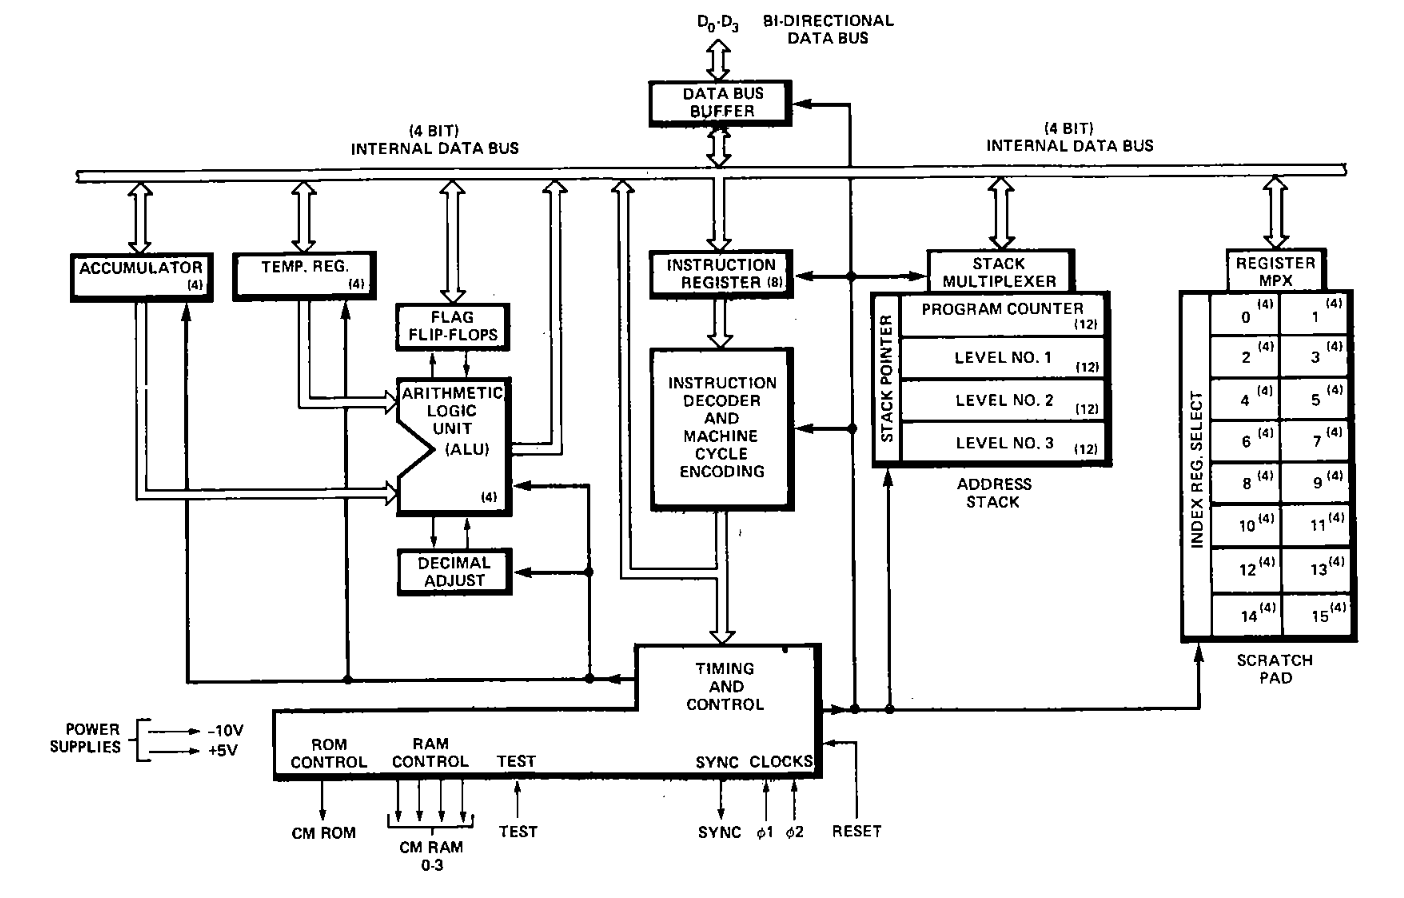
\includegraphics[width=0.88\textwidth]{diagrama}\\[0.6em]
        {\small\textit{Diagrama de bloques del procesador Intel~4004}}
    \end{center}
}
\keywords{spanish}{
    VHDL; Intel 4004; FPGA; Artix-7; Arquitectura de computadores
}

\newacronym{vhdl}{VHDL}{\textit{Very High Speed Integrated Circuit Hardware Description Language}}
\newacronym{fpga}{FPGA}{\textit{Field Programmable Gate Array}}
\newacronym{cpu}{CPU}{Unidad Central de Proceso}
\newacronym{alu}{ALU}{Unidad Aritmético-Lógica}
\newacronym{ir}{IR}{Registro de Instrucción}
\newacronym{pc}{PC}{\textit{Program Counter}}
\newacronym{bcd}{BCD}{\textit{Binary Coded Decimal}}
\newacronym{phr}{PHR}{Programación de Hardware Reconfigurable}
\newacronym{ff}{FF}{\textit{Flip-Flop}}
\newacronym{fsm}{FSM}{\textit{Finite State Machine}}
\newacronym{oe}{OE}{\textit{Output Enable}}
\newacronym{bram}{BRAM}{\textit{Block RAM}}
\newacronym{soc}{SoC}{\textit{System on Chip}}

\newglossaryentry{bus-interno}{
    name=bus interno,
    description={Bus de datos de 4~bits que interconecta todos los bloques
        funcionales internos de la CPU}}
\newglossaryentry{nibble}{
    name=nibble,
    description={Grupo de 4~bits}}
\newglossaryentry{scratchpad}{
    name=scratchpad,
    description={Banco de 16~registros de 4~bits internos (R0--R15)}}
\newglossaryentry{stack}{
    name=pila de direcciones,
    description={Estructura de tres niveles de 12~bits para llamadas a subrutina}}

\newcommand{\vhdlfile}[1]{%
    \par\noindent{\small\sffamily\color{gray}Fichero: \texttt{#1}}\par\smallskip
}

\addbibresource{references.bib}

\begin{document}

% ======================================================================
\chapter{Introducción}
\label{ch:introduccion}
% ======================================================================

El Intel~4004, lanzado en noviembre de 1971, fue el primer \acrfull{cpu}
comercial integrado en un único circuito integrado.  Diseñado para la
calculadora de escritorio Busicom 141-PF, estableció las bases de la industria
del microprocesador con apenas 2\,300~transistores, una arquitectura de 4~bits
y una frecuencia máxima de 740~kHz.

El objetivo de este proyecto, enmarcado en la asignatura \acrfull{phr} del
Grado en Ingeniería de Computadores de la \textit{Escuela Técnica Superior de
Ingeniería de Sistemas Informáticos} de la \textit{Universidad Politécnica de
Madrid}, es reimplementar este procesador en \acrshort{vhdl} y sintetizarlo
sobre una \acrshort{fpga} Artix-7 Basys~3.

\section{Objetivos}

\begin{enumerate}
    \item Estudiar la especificación técnica original del Intel~4004.
    \item Diseñar la arquitectura en \acrshort{vhdl} dividida en bloques
        funcionales fieles al diagrama de la especificación.
    \item Implementar un subconjunto funcional del juego de instrucciones
        suficiente para ejecutar la aplicación de demostración.
    \item Verificar el diseño mediante simulación con testbenches.
    \item Sintetizar e implementar el diseño sobre la Basys~3 Artix-7.
\end{enumerate}

\section{Alcance de la implementación}

El Intel~4004 original define 46~instrucciones.  Esta implementación cubre
el subconjunto necesario para la aplicación de demostración: aritmética
(\texttt{ADD}, \texttt{SUB}, \texttt{INC}, \texttt{DAA}), carga de registros
(\texttt{LD}, \texttt{LDM}, \texttt{XCH}, \texttt{FIM}), control de flujo
(\texttt{JUN}, \texttt{JMS}, \texttt{JCN}, \texttt{BBL}), acceso al banco de
registros (\texttt{SRC}), entrada/salida con ROM (\texttt{RDR}, \texttt{WRR})
y manipulación de flags (\texttt{CLC}, \texttt{CMC}, \texttt{CLB}).  Quedan
fuera del alcance las instrucciones de acceso a la RAM~4002 y otros grupos
de control; véase la sección~\ref{s:limitaciones}.

\section{Estructura de la memoria}

El capítulo~\ref{ch:estado-cuestion} describe la arquitectura del Intel~4004.
El capítulo~\ref{ch:metodologia} presenta la metodología seguida.  El
capítulo~\ref{ch:diseno} contiene el núcleo técnico del trabajo, recorriendo
los bloques \acrshort{vhdl} en orden de dependencia ascendente: desde las
primitivas hasta el integrador top-level.  Los capítulos~\ref{ch:verificacion}
e~\ref{ch:implementacion} recogen la verificación y la síntesis sobre hardware.

% ======================================================================
\chapter{Estado de la cuestión}
\label{ch:estado-cuestion}
% ======================================================================

\section{El procesador Intel 4004}

El Intel~4004 fue diseñado por Federico Faggin, Marcian Hoff, Stanley Mazor
y Masatoshi Shima.  Sus características principales son:

\begin{itemize}
    \item Bus de datos externo bidireccional de 4~bits (D0--D3), multiplexado
        en el tiempo para transportar tanto datos como los tres \glspl{nibble}
        de la dirección de 12~bits.
    \item Acumulador de 4~bits y su \acrshort{alu} asociada.
    \item Banco de 16~registros internos (\gls{scratchpad}) de 4~bits,
        agrupables en 8~pares de 8~bits.
    \item \Gls{stack} de tres niveles de 12~bits; el \acrshort{pc} es siempre
        la cima de la pila.
    \item Ciclo de máquina de 8~fases (A1--A3, M1--M2, X1--X3) controlado
        por dos relojes en cuadratura no solapados ($\phi_1$, $\phi_2$).
    \item Señales de control: \texttt{SYNC}, \texttt{CM-ROM} y
        \texttt{CM-RAM[3:0]}.
    \item Juego de 46~instrucciones de 8~bits (16~bits para instrucciones de
        dos ciclos de máquina).
\end{itemize}

\section{Herramientas utilizadas}

\begin{itemize}
    \item \textit{Vivado Design Suite} 2024 de Xilinx/AMD.
    \item \acrshort{vhdl}-93 como lenguaje de descripción hardware.
    \item Placa Basys~3 (Artix-7 XC7A35TICPG236-1L) como destino hardware.
\end{itemize}

% ======================================================================
\chapter{Metodología}
\label{ch:metodologia}
% ======================================================================

El proyecto sigue la metodología de diseño de la asignatura \acrshort{phr}:

\bigskip
\begin{center}
    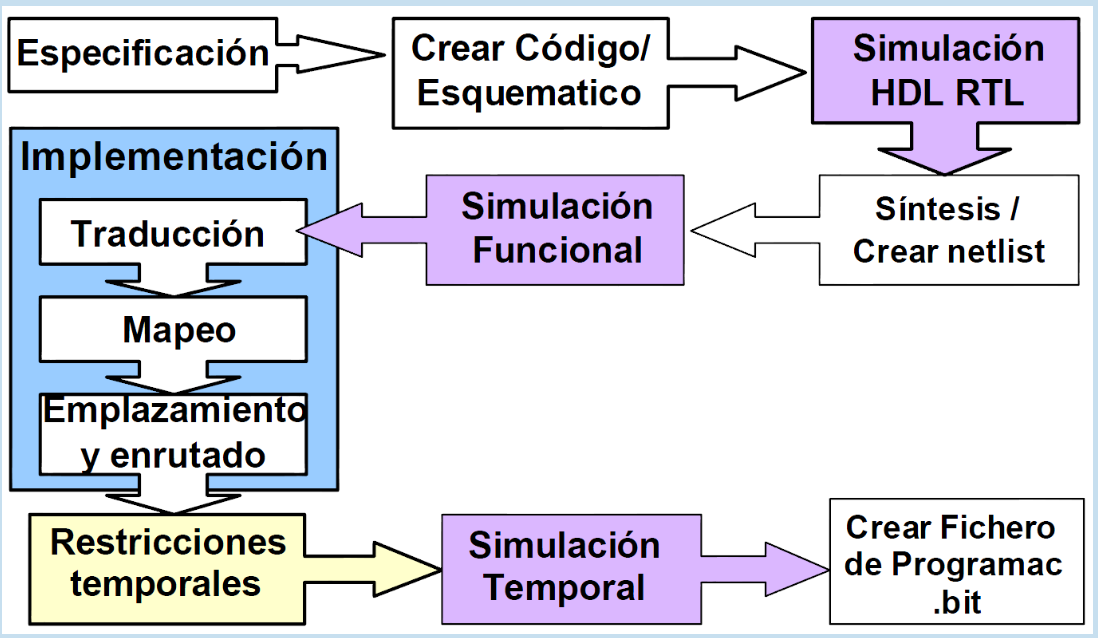
\includegraphics[width=0.82\textwidth]{metodologia}\\[0.6em]
    {\small\textit{Fases de la metodología de diseño de la asignatura \acrshort{phr}}}
\end{center}

\bigskip
El proceso comenzó con el análisis de la especificación técnica del
Intel~4004, identificando los bloques funcionales y el subconjunto de
instrucciones a implementar.  A continuación se diseñó la jerarquía de
ficheros \acrshort{vhdl}, un fichero por bloque funcional.  Cada bloque se
verificó de forma individual mediante testbench antes de integrarse en el
nivel superior.  Por último, se sintetizó e implementó el diseño completo
sobre la Basys~3.

% ======================================================================
\chapter{Diseño}
\label{ch:diseno}
% ======================================================================

Este capítulo recorre los bloques \acrshort{vhdl} del diseño en orden de
dependencia ascendente: comenzando por las constantes globales y las
primitivas de hardware, avanzando a través de la ruta de datos, la pila, el
bus y la unidad de control, hasta llegar al fichero integrador top-level y al
\acrshort{soc} que lo conecta con la placa física.

% ----------------------------------------------------------------------
\section{Filosofía de diseño y paquete global}
\label{s:estructura}
% ----------------------------------------------------------------------

\subsection{Arquitectura estructural jerárquica}

La primera decisión del proyecto fue adoptar una \textbf{arquitectura
puramente estructural} en todos los niveles de la jerarquía: cada bloque
funcional instancia componentes de nivel inferior hasta llegar, en la base,
a primitivas de \acrfull{ff} individuales.

Esta elección responde a tres criterios.  Primero, la síntesis es
completamente predecible: cada \texttt{registro\_4b} se convierte en cuatro
primitivos \texttt{FDRE} de la Artix-7, sin inferencias implícitas.  Segundo,
la verificación es incremental: cada primitiva puede simularse de forma
aislada antes de integrarse en el bloque superior.  Tercero, existe una
correspondencia directa entre el diagrama de bloques de la especificación y
la jerarquía de ficheros \acrshort{vhdl}, facilitando la trazabilidad.

\subsection{Paquete de constantes}
\vhdlfile{pkg\_4004.vhd}

El paquete \texttt{pkg\_4004} centraliza las constantes globales.  Todos
los módulos lo importan con \texttt{use work.pkg\_4004.all}.

\begin{lstlisting}[language=VHDL, caption={Contenido del paquete \texttt{pkg\_4004}},
    label=lst:pkg4004]
constant BUS_W     : integer := 4;
constant BUS_CERO  : std_logic_vector(BUS_W-1 downto 0) := "0000";
constant BUS_ERROR : std_logic_vector(BUS_W-1 downto 0) := "XXXX";
\end{lstlisting}

\texttt{BUS\_W} define el ancho del \gls{bus-interno}; todos los vectores
de datos se dimensionan con ella.  \texttt{BUS\_ERROR} sirve para detectar
colisiones de bus en simulación: si dos fuentes conducen el bus
simultáneamente, la salida del multiplexor central toma el valor
\texttt{"XXXX"}, inmediatamente visible en el visor de señales de Vivado.

% ----------------------------------------------------------------------
\clearpage
\section{Primitivas de hardware}
\label{s:primitivas}
% ----------------------------------------------------------------------

En la base de la jerarquía se encuentran tres primitivas que representan los
elementos de memoria más simples.

\subsection{\textit{Flip-flop} D con enable}
\label{ss:d-ff-en}
\vhdlfile{d\_ff\_en.vhd}

Es el elemento de memoria fundamental del diseño.  Prácticamente todos los
registros de la \acrshort{cpu} se construyen como matrices de instancias de
esta entidad.  Implementa un \acrfull{ff} tipo~D síncrono con reset asíncrono
activo alto y señal de habilitación.

\begin{table}[H]
\centering
\caption{Puertos de la entidad \texttt{d\_ff\_en}}
\label{tab:d-ff-en}
\begin{tabularx}{\textwidth}{@{}llcX@{}}
\toprule
\textbf{Puerto} & \textbf{Dir.} & \textbf{Bits} & \textbf{Descripción} \\
\midrule
\texttt{clk}   & in  & 1 & Reloj; captura en flanco de subida \\
\texttt{reset} & in  & 1 & Reset asíncrono activo alto \\
\texttt{en}    & in  & 1 & Habilitación síncrona \\
\texttt{d}     & in  & 1 & Dato de entrada \\
\texttt{q}     & out & 1 & Salida del \acrshort{ff} \\
\bottomrule
\end{tabularx}
\end{table}

La arquitectura \texttt{Behavioral} implementa el proceso sensible a
\texttt{clk} y \texttt{reset}: si reset está activo, la salida se lleva a
\texttt{'0'} de forma asíncrona; en el flanco de subida, si \texttt{en = '1'},
se captura \texttt{d}.  El sintetizador mapea este patrón directamente sobre
un primitivo \texttt{FDRE} de la Artix-7.

\subsection{Registros de 4 y 12 bits}
\label{ss:registros}
\vhdlfile{registro\_4b.vhd, registro\_12b.vhd}

Ambos se implementan con una sentencia \texttt{GENERATE} que instancia $N$
copias de \texttt{d\_ff\_en} en paralelo ($N = 4$ ó $N = 12$).

\begin{table}[H]
\centering
\caption{Puertos del \texttt{registro\_4b} (análogos en \texttt{registro\_12b})}
\label{tab:registro-4b}
\begin{tabularx}{\textwidth}{@{}llcX@{}}
\toprule
\textbf{Puerto} & \textbf{Dir.} & \textbf{Bits} & \textbf{Descripción} \\
\midrule
\texttt{clk}    & in  & 1      & Reloj del sistema \\
\texttt{R}      & in  & 1      & Reset asíncrono activo alto \\
\texttt{E}      & in  & 1      & Enable síncrono de escritura \\
\texttt{D\_in}  & in  & 4 (12) & Dato a cargar cuando \texttt{E = '1'} \\
\texttt{Q\_out} & out & 4 (12) & Dato almacenado \\
\bottomrule
\end{tabularx}
\end{table}

\subsection{\textit{Flip-flop} JK}
\label{ss:ff-jk}
\vhdlfile{flipflopJK.vhd}

\acrshort{ff} de tipo~JK utilizado exclusivamente en el puntero de pila
(sección~\ref{ss:puntero-stack}).  Proporciona las salidas directa
(\texttt{q}) y complementada (\texttt{notq}).

\begin{table}[H]
\centering
\caption{Puertos de la entidad \texttt{flipflopJK}}
\label{tab:ff-jk}
\begin{tabularx}{\textwidth}{@{}llcX@{}}
\toprule
\textbf{Puerto} & \textbf{Dir.} & \textbf{Bits} & \textbf{Descripción} \\
\midrule
\texttt{j}    & in  & 1 & Entrada J \\
\texttt{k}    & in  & 1 & Entrada K \\
\texttt{r}    & in  & 1 & Reset asíncrono activo alto \\
\texttt{clk}  & in  & 1 & Reloj de captura (flanco de subida) \\
\texttt{q}    & out & 1 & Salida directa \\
\texttt{notq} & out & 1 & Salida complementada \\
\bottomrule
\end{tabularx}
\end{table}

% ----------------------------------------------------------------------
\section{Ruta de datos}
\label{s:ruta-datos}
% ----------------------------------------------------------------------

\subsection{Acumulador}
\label{ss:accumulator}
\vhdlfile{accumulator.vhd}

El acumulador almacena el primer operando y el resultado de toda operación
aritmética o lógica.  Se implementa como un \textit{wrapper} sobre
\texttt{registro\_4b}: la entidad \texttt{accumulator} no añade lógica propia,
ya que el acumulador del Intel~4004 no tiene circuitería especial asociada.
Su existencia como entidad separada responde a razones de legibilidad y
trazabilidad con la especificación.

\begin{table}[H]
\centering
\caption{Puertos de la entidad \texttt{accumulator}}
\label{tab:accumulator}
\begin{tabularx}{\textwidth}{@{}llcX@{}}
\toprule
\textbf{Puerto}  & \textbf{Dir.} & \textbf{Bits} & \textbf{Descripción} \\
\midrule
\texttt{clk}     & in  & 1 & Reloj del sistema \\
\texttt{reset}   & in  & 1 & Reset asíncrono \\
\texttt{load\_en}& in  & 1 & Señal de escritura desde \texttt{timing\_and\_control} \\
\texttt{d\_in}   & in  & 4 & Dato a cargar (del \gls{bus-interno}) \\
\texttt{q\_out}  & out & 4 & Contenido actual (hacia la \acrshort{alu} y el bus) \\
\bottomrule
\end{tabularx}
\end{table}

\subsection{Registro temporal}
\label{ss:temp-register}
\vhdlfile{temp\_register.vhd}

El registro temporal almacena el segundo operando de la \acrshort{alu}.
Durante la fase~X1, el controlador carga en él el valor del registro fuente
del \gls{scratchpad}; en la fase~X2, ese valor pasa a la entrada~B de la
\acrshort{alu}.  Su implementación es idéntica a la del acumulador: un
\textit{wrapper} sobre \texttt{registro\_4b}.

\subsection{Registro de instrucción}
\label{ss:ir}
\vhdlfile{instruction\_register.vhd}

El \acrfull{ir} captura la instrucción de dos \glspl{nibble} procedentes del
\gls{bus-interno} durante las fases de búsqueda.  Se implementa de forma
estructural como ocho instancias de \texttt{d\_ff\_en} organizadas en dos
grupos de cuatro mediante \texttt{GENERATE}: el grupo alto (bits~7--4) se
captura en la fase~M1 cuando \texttt{load\_high = '1'}; el grupo bajo
(bits~3--0) en la fase~M2 cuando \texttt{load\_low = '1'}.

\begin{table}[H]
\centering
\caption{Puertos de la entidad \texttt{instruction\_register}}
\label{tab:ir}
\begin{tabularx}{\textwidth}{@{}llcX@{}}
\toprule
\textbf{Puerto}     & \textbf{Dir.} & \textbf{Bits} & \textbf{Descripción} \\
\midrule
\texttt{clk}        & in  & 1 & Reloj del sistema \\
\texttt{reset}      & in  & 1 & Reset asíncrono \\
\texttt{load\_high} & in  & 1 & Carga nibble alto (activo en M1) \\
\texttt{load\_low}  & in  & 1 & Carga nibble bajo (activo en M2) \\
\texttt{bus\_in}    & in  & 4 & Dato del \gls{bus-interno} \\
\texttt{instr\_out} & out & 8 & Instrucción completa hacia el decodificador \\
\bottomrule
\end{tabularx}
\end{table}

La señal \texttt{disable\_ir} (gestionada en \texttt{cpu\_4004\_top}) impide
que el \acrshort{ir} capture un nuevo opcode durante el segundo ciclo de
instrucciones de 2~bytes, preservando el opcode del primer byte durante la
ejecución.

\subsection{Registros de flags}
\label{ss:flags}
\vhdlfile{flag\_flip\_flops.vhd}

Almacena el vector de estado de la \acrshort{cpu}.  La lógica de formación
de la entrada (\texttt{d\_in}) se describe en \texttt{cpu\_4004\_top}:

\begin{itemize}
    \item \textbf{Bit~0, Carry}: recibe el acarreo de la \acrshort{alu} en
        operaciones aritméticas, \texttt{'0'} en \texttt{CLC} y \texttt{CLB},
        o el complemento del carry actual en \texttt{CMC}.
    \item \textbf{Bit~1, Test}: conectado directamente al pin físico
        \texttt{test\_pin}.
    \item \textbf{Bits 2--3}: reservados a \texttt{'0'}.
\end{itemize}

\begin{table}[H]
\centering
\caption{Puertos de la entidad \texttt{flag\_flip\_flops}}
\label{tab:flags}
\begin{tabularx}{\textwidth}{@{}llcX@{}}
\toprule
\textbf{Puerto}    & \textbf{Dir.} & \textbf{Bits} & \textbf{Descripción} \\
\midrule
\texttt{clk}       & in  & 1 & Reloj del sistema \\
\texttt{reset}     & in  & 1 & Reset asíncrono \\
\texttt{load\_en}  & in  & 1 & Señal de escritura \\
\texttt{d\_in}     & in  & 4 & Valor a cargar \\
\texttt{q\_out}    & out & 4 & Estado actual de los flags \\
\texttt{flags\_oe} & in  & 1 & \acrshort{oe} hacia el \gls{bus-interno} \\
\bottomrule
\end{tabularx}
\end{table}

\subsection{Unidad Aritmético-Lógica}
\label{ss:alu}
\vhdlfile{alu.vhd}

La \acrfull{alu} realiza todas las operaciones aritméticas y lógicas.  Su
arquitectura \texttt{Combinational} no contiene ningún elemento de memoria;
el resultado está disponible de forma continua.

\begin{table}[H]
\centering
\caption{Puertos de la entidad \texttt{alu}}
\label{tab:alu}
\begin{tabularx}{\textwidth}{@{}llcX@{}}
\toprule
\textbf{Puerto}     & \textbf{Dir.} & \textbf{Bits} & \textbf{Descripción} \\
\midrule
\texttt{A\_in}        & in  & 4 & Primer operando (acumulador o registro de scratchpad) \\
\texttt{B\_in}        & in  & 4 & Segundo operando (temp. register o ajuste decimal) \\
\texttt{carry\_in}    & in  & 1 & Acarreo de entrada (\texttt{flags\_out[0]}) \\
\texttt{op}           & in  & 3 & Código de operación \\
\texttt{result\_out}  & out & 4 & Resultado \\
\texttt{carry\_out}   & out & 1 & Acarreo de salida \\
\texttt{zero\_flag}   & out & 1 & Activo si \texttt{result\_out = "0000"} \\
\bottomrule
\end{tabularx}
\end{table}

\begin{table}[H]
\centering
\caption{Operaciones de la \acrshort{alu}}
\label{tab:alu-ops}
\begin{tabularx}{\textwidth}{@{}clX@{}}
\toprule
\textbf{\texttt{op}} & \textbf{Operación} & \textbf{Descripción} \\
\midrule
\texttt{000} & ADD  & $A + B + C_{in}$ \\
\texttt{001} & SUB  & $A + \overline{B} + C_{in}$ (complemento a~1, fiel al 4004) \\
\texttt{010} & AND  & $A$ \textsc{and} $B$ \\
\texttt{011} & OR   & $A$ \textsc{or} $B$ \\
\texttt{100} & XOR  & $A$ \textsc{xor} $B$ \\
\texttt{101} & PASS & Pasa $A$ sin modificar (valor por defecto) \\
\texttt{110} & INC  & $A + 1$ \\
\bottomrule
\end{tabularx}
\end{table}

Los tres resultados de mayor coste (ADD, SUB, INC) se calculan siempre en
paralelo mediante señales intermedias de 5~bits, y un proceso \texttt{case}
final selecciona cuál se propaga a la salida.  El bit de acarreo es el
bit~4 de la señal de 5~bits correspondiente.

La entrada~B de la \acrshort{alu} proviene de un multiplexor en
\texttt{cpu\_4004\_top}: normalmente conecta con \texttt{temp\_register},
pero cuando \texttt{ctrl\_alu\_b\_mux = '1'} conecta con la salida del bloque
de ajuste decimal.

\subsection{Ajuste decimal}
\label{ss:decimal-adjust}
\vhdlfile{decimal\_adjust.vhd}

Bloque combinacional que calcula la corrección \acrshort{bcd} para
\texttt{DAA}.  Si el acarreo está activo o el acumulador supera~9, la
corrección es \texttt{0110} (+6); en caso contrario es \texttt{0000}.

\begin{table}[H]
\centering
\caption{Puertos de la entidad \texttt{decimal\_adjust}}
\label{tab:decimal-adjust}
\begin{tabularx}{\textwidth}{@{}llcX@{}}
\toprule
\textbf{Puerto}    & \textbf{Dir.} & \textbf{Bits} & \textbf{Descripción} \\
\midrule
\texttt{acc\_in}   & in  & 4 & Contenido actual del acumulador \\
\texttt{carry\_in} & in  & 1 & Acarreo actual \\
\texttt{adj\_out}  & out & 4 & Corrección a sumar (\texttt{0000} ó \texttt{0110}) \\
\bottomrule
\end{tabularx}
\end{table}

\subsection{Banco de registros (\textit{scratchpad})}
\label{ss:scratchpad}
\vhdlfile{scratch\_pad.vhd, mtx\_scratchpad.vhd}

El \gls{scratchpad} implementa los 16~registros de propósito general de 4~bits
del Intel~4004 (R0--R15), agrupables en 8~pares de 8~bits.  La arquitectura
\texttt{Structural} instancia 16~copias de \texttt{registro\_4b} y un
multiplexor 16:1 (\texttt{mtx\_scratchpad}) para leer el registro seleccionado.

\begin{table}[H]
\centering
\caption{Puertos de la entidad \texttt{scratch\_pad}}
\label{tab:scratchpad}
\begin{tabularx}{\textwidth}{@{}llcX@{}}
\toprule
\textbf{Puerto}     & \textbf{Dir.} & \textbf{Bits} & \textbf{Descripción} \\
\midrule
\texttt{clk\_r}     & in  & 1 & Reloj del sistema \\
\texttt{rst\_r}     & in  & 1 & Reset asíncrono \\
\texttt{w\_e}       & in  & 1 & Write enable \\
\texttt{pair\_mode} & in  & 1 & \texttt{'1'}: acceso en par de 8~bits \\
\texttt{address}    & in  & 4 & Dirección del registro (0--15) \\
\texttt{data\_in}   & in  & 8 & Dato a escribir \\
\texttt{data\_out}  & out & 8 & Dato leído \\
\bottomrule
\end{tabularx}
\end{table}

En modo par (\texttt{pair\_mode = '1'}), se activan simultáneamente el
registro par e impar: el par recibe \texttt{data\_in[7:4]} y el impar
\texttt{data\_in[3:0]}, modelando las instrucciones \texttt{FIM} (carga de
un par con inmediato de 8~bits) y \texttt{SRC} (envío de dirección de 8~bits
al bus externo en dos \glspl{nibble}).

El direccionamiento durante instrucciones de par se gestiona en
\texttt{cpu\_4004\_top}: la lógica selecciona el registro par o impar según
la fase del ciclo de máquina (\texttt{t\_state}).

% ----------------------------------------------------------------------
\section{Pila de direcciones}
\label{s:stack}
% ----------------------------------------------------------------------

\vhdlfile{stack\_3L.vhd}

La \gls{stack} implementa los tres niveles de 12~bits del Intel~4004.  A
diferencia de un diseño convencional donde el \acrshort{pc} es un registro
separado, en el 4004 el \acrshort{pc} \textbf{es siempre la cima de la pila}.
Se implementa como cuatro registros de 12~bits (\texttt{registro\_12b}) con
un puntero de pila de 2~bits que selecciona el nivel activo.

\begin{table}[H]
\centering
\caption{Puertos de la entidad \texttt{stack\_3L}}
\label{tab:stack}
\begin{tabularx}{\textwidth}{@{}llcX@{}}
\toprule
\textbf{Puerto}       & \textbf{Dir.} & \textbf{Bits} & \textbf{Descripción} \\
\midrule
\texttt{Clk\_s}       & in  & 1  & Reloj del sistema \\
\texttt{sp\_clk}      & in  & 1  & Reloj del puntero (activo solo en JMS y BBL) \\
\texttt{U\_D\_s}      & in  & 1  & Dirección: \texttt{'0'} push (JMS), \texttt{'1'} pop (BBL) \\
\texttt{D\_12\_s}     & in  & 12 & Dirección a escribir (PC+1 o dirección de salto) \\
\texttt{E\_s}         & in  & 1  & Enable de escritura \\
\texttt{R\_s}         & in  & 1  & Reset \\
\texttt{oe\_s}        & in  & 1  & \acrshort{oe} hacia el \gls{bus-interno} \\
\texttt{fase\_s}      & in  & 2  & Fase del reloj para serialización \\
\texttt{sal\_4\_stck} & out & 4  & \gls{nibble} serializado hacia el \gls{bus-interno} \\
\texttt{PC\_out}      & out & 12 & Valor actual del \acrshort{pc} \\
\bottomrule
\end{tabularx}
\end{table}

La entrada de datos (\texttt{stack\_in\_12b}) se decide en
\texttt{cpu\_4004\_top}: si la instrucción es un salto efectivo se carga la
dirección destino; en caso contrario se carga \texttt{PC + 1}.

\subsubsection{Puntero de pila}
\label{ss:puntero-stack}
\vhdlfile{puntero\_stack.vhd}

Contador bidireccional de 2~bits construido con dos \acrshort{ff} tipo~JK
(\texttt{flipflopJK}).  Cuando \texttt{up\_down = '1'} el puntero avanza
(push en \texttt{JMS}); cuando es \texttt{'0'} retrocede (pop en
\texttt{BBL}).  El reloj del puntero (\texttt{sp\_clk}) solo conmuta durante
instrucciones de llamada o retorno.

\subsubsection{Multiplexor de pila con serialización}
\label{ss:mtx-stack}
\vhdlfile{mtx\_stack.vhd}

Selecciona el nivel activo y serializa su contenido de 12~bits en tres
\glspl{nibble} de 4~bits para volcarlo al \gls{bus-interno} durante A1, A2
y A3:

\begin{lstlisting}[language=VHDL, caption={Serialización del PC en \texttt{mtx\_stack}},
    label=lst:mtx-stack-ser]
when "00" => y <= reg_activo(3  downto 0);   -- A1: nibble bajo
when "01" => y <= reg_activo(7  downto 4);   -- A2: nibble medio
when "10" => y <= reg_activo(11 downto 8);   -- A3: nibble alto
\end{lstlisting}

% ----------------------------------------------------------------------
\section{Bus interno y buffer de datos}
\label{s:interfaz}
% ----------------------------------------------------------------------

\subsection{Bus interno --- multiplexor central}
\label{ss:bus-interno}
\vhdlfile{bus\_interno\_mux.vhd}

El \gls{bus-interno} de 4~bits es el canal de comunicación entre todos los
bloques funcionales.  Se implementa como un \textbf{multiplexor centralizado}
en lugar de un bus triestado interno.

En \acrshort{vhdl} lo más natural sería usar señales \texttt{std\_logic} con
alta impedancia \texttt{'Z'}.  Sin embargo, los recursos internos de la
Artix-7 no disponen de buffers triestado en la \textit{fabric}; el
sintetizador los convertiría igualmente en multiplexores, pero de forma
implícita y menos predecible.  El multiplexor explícito ofrece además
detección de colisiones en simulación mediante \texttt{BUS\_ERROR = "XXXX"}.

\begin{table}[H]
\centering
\caption{Fuentes del \texttt{bus\_interno\_mux} (cada una con su señal \texttt{\_oe})}
\label{tab:bus-mux}
\begin{tabularx}{\textwidth}{@{}lX@{}}
\toprule
\textbf{Fuente}        & \textbf{Descripción} \\
\midrule
\texttt{acc\_out}      & Acumulador \\
\texttt{tmp\_reg\_out} & Registro temporal \\
\texttt{flags\_out}    & Registros de flags \\
\texttt{alu\_out}      & Resultado de la \acrshort{alu} \\
\texttt{decoder\_out}  & Decodificador (inmediatos LDM/BBL) \\
\texttt{stack\_out}    & Pila de direcciones (PC serializado) \\
\texttt{reg\_mux\_out} & \textit{Scratchpad} \\
\texttt{ext\_buf\_out} & Buffer de bus externo (instrucción de la ROM) \\
\bottomrule
\end{tabularx}
\end{table}

\subsection{Buffer de bus de datos}
\label{ss:data-bus-buffer}
\vhdlfile{data\_bus\_buffer.vhd}

Gestiona la comunicación bidireccional con el pin físico \texttt{D\_bus}
(D0--D3).  Cuando \texttt{dir\_out = '0'}, el CPU vuelca datos al exterior
(fases A1--A3: la dirección del \acrshort{pc} va hacia la ROM).  Cuando
\texttt{dir\_out = '1'}, el pin externo alimenta el \gls{bus-interno}
(fases M1--M2: la ROM entrega la instrucción).

\begin{table}[H]
\centering
\caption{Puertos de la entidad \texttt{data\_bus\_buffer}}
\label{tab:dbb}
\begin{tabularx}{\textwidth}{@{}llcX@{}}
\toprule
\textbf{Puerto}             & \textbf{Dir.}  & \textbf{Bits} & \textbf{Descripción} \\
\midrule
\texttt{internal\_bus\_in}  & in    & 4 & Dato del bus interno (hacia el exterior) \\
\texttt{internal\_bus\_out} & out   & 4 & Dato hacia el bus interno (desde el exterior) \\
\texttt{dir\_out}           & in    & 1 & \texttt{'1'}: CPU escribe en \texttt{D\_bus} \\
\texttt{data\_bus\_ext}     & inout & 4 & Pin bidireccional D0--D3 \\
\bottomrule
\end{tabularx}
\end{table}

A diferencia del bus interno, aquí el triestado es correcto y necesario:
\texttt{data\_bus\_ext} es un pin físico del encapsulado, y los pines
\texttt{IOB} de la Artix-7 sí disponen de buffers triestado reales.

% ----------------------------------------------------------------------
\section{Unidad de control}
\label{s:control}
% ----------------------------------------------------------------------

\subsection{Decodificador de instrucciones}
\label{ss:decoder}
\vhdlfile{instruction\_decoder.vhd}

El decodificador traduce el byte de instrucción almacenado en el \acrshort{ir}
en señales de control combinacionales para la unidad de temporización.

\begin{table}[H]
\centering
\caption{Puertos de la entidad \texttt{instruction\_decoder} conectados en \texttt{cpu\_4004\_top}}
\label{tab:decoder}
\begin{tabularx}{\textwidth}{@{}llcX@{}}
\toprule
\textbf{Puerto}    & \textbf{Dir.} & \textbf{Bits} & \textbf{Descripción} \\
\midrule
\texttt{ir\_in}      & in  & 8  & Byte de instrucción actual \\
\texttt{inst\_group} & out & 16 & Codificación One-Hot del grupo de instrucción \\
\texttt{is\_2byte}   & out & 1  & Instrucción de 2 ciclos (JUN, JMS, JCN, FIM) \\
\texttt{bus\_out}    & out & 4  & Dato inmediato (nibble bajo, para LDM y BBL) \\
\texttt{out\_en}     & out & 1  & \acrshort{oe} del inmediato hacia el bus interno \\
\bottomrule
\end{tabularx}
\end{table}

La entidad define además puertos indicadores individuales (\texttt{is\_daa},
\texttt{is\_tcs}, \texttt{is\_rdr}, \texttt{is\_wrr}, \texttt{is\_wmp},
\texttt{is\_clc}, \texttt{is\_clb}, \texttt{is\_cmc}), pero en
\texttt{cpu\_4004\_top} no se conectan: el bloque
\texttt{timing\_and\_control} infiere esa misma información combinando la
señal \texttt{inst\_group} con el contenido de \texttt{ir\_in}, que recibe
directamente, por lo que los indicadores separados resultan redundantes a
nivel de integración.

La decodificación principal se realiza con un \texttt{case} sobre el nibble
alto del opcode (\texttt{ir\_in[7:4]}), generando una codificación
\textbf{One-Hot} de 16~bits en \texttt{inst\_group}: el bit~$n$ activo
indica que la instrucción pertenece al grupo con opcode alto $n$.

Las instrucciones \texttt{LDM} (grupo~13) y \texttt{BBL} (grupo~7) colocan
su dato inmediato directamente en \texttt{bus\_out} (\texttt{ir\_in[3:0]})
y activan \texttt{out\_en} para que el valor aparezca en el \gls{bus-interno}
sin ningún registro adicional.

\subsection{Temporización y control}
\label{ss:timing-control}
\vhdlfile{timing\_and\_control.vhd}

El bloque \texttt{timing\_and\_control} es el corazón de la unidad de
control.  Implementa la \acrfull{fsm} de 8~estados del ciclo de máquina y
genera todas las señales de control del \textit{datapath}.

La \acrshort{fsm} se describe con arquitectura \texttt{Behavioral}: un proceso
secuencial incrementa un contador de 3~bits en cada flanco de subida de
\texttt{clk\_ph1}, ciclando de \texttt{000} a \texttt{111}.  Un segundo
proceso combinacional produce las señales de salida mediante un \texttt{case}.

\begin{table}[H]
\centering
\caption{Fases del ciclo de máquina y función de cada una}
\label{tab:fases}
\begin{tabularx}{\textwidth}{@{}llX@{}}
\toprule
\textbf{Estado} & \textbf{Fase} & \textbf{Función} \\
\midrule
\texttt{000} & A1 & \texttt{sync = '1'}; nibble bajo del PC al bus externo \\
\texttt{001} & A2 & Nibble medio del PC al bus externo \\
\texttt{010} & A3 & Nibble alto del PC; activa \texttt{cm\_rom} \\
\texttt{011} & M1 & Captura nibble alto de la instrucción desde la ROM \\
\texttt{100} & M2 & Captura nibble bajo de la instrucción desde la ROM \\
\texttt{101} & X1 & Primera fase de ejecución (lectura de operando) \\
\texttt{110} & X2 & Segunda fase de ejecución (operación ALU / escritura) \\
\texttt{111} & X3 & Tercera fase de ejecución (actualización del PC) \\
\bottomrule
\end{tabularx}
\end{table}

Las señales \texttt{inst\_group} y \texttt{current\_frag} procedentes del
decodificador determinan qué señales de control se activan durante X1--X3.
La señal \texttt{current\_frag} distingue el primer del segundo ciclo de
máquina de instrucciones de 2~bytes.

% ----------------------------------------------------------------------
\section{Integración: \textit{top-level} de la CPU}
\label{s:integracion}
% ----------------------------------------------------------------------

\vhdlfile{cpu\_4004\_top.vhd}

El fichero \texttt{cpu\_4004\_top.vhd} ensambla todos los bloques descritos
en las secciones anteriores mediante cláusulas \texttt{port map}.  No contiene
lógica funcional propia salvo tres elementos de \textit{glue logic} que no
pertenecen a ningún bloque individual:

\begin{itemize}
    \item \textbf{Bypass de INC}: la entrada~A de la \acrshort{alu} se
        conecta normalmente al acumulador, pero durante \texttt{INC} se
        redirige a la salida del \gls{scratchpad} para incrementar un
        registro de índice directamente, sin alterar el acumulador.

    \item \textbf{Fix de DAA}: el carry de entrada a la \acrshort{alu} se
        fuerza a \texttt{'0'} durante \texttt{DAA} para que el ajuste
        decimal no incluya el carry antiguo como sumando adicional.

    \item \textbf{Lógica de instrucciones de 2~bytes}: un proceso secuencial
        gestiona \texttt{current\_frag} y \texttt{disable\_ir} para controlar
        la ejecución en dos ciclos de \texttt{JUN}, \texttt{JMS}, \texttt{JCN}
        y \texttt{FIM}.  Captura el segundo byte en \texttt{second\_byte\_reg}
        y evalúa la condición de salto para \texttt{JCN} comparando el
        acumulador, el carry y el \texttt{test\_pin} con las condiciones
        codificadas en el nibble bajo del opcode.
\end{itemize}

La entidad expone exactamente los pines físicos del DIP-16 del Intel~4004
original: \texttt{clk\_ph1}, \texttt{clk\_ph2}, \texttt{reset},
\texttt{test\_pin}, \texttt{sync}, \texttt{cm\_rom}, \texttt{cm\_ram[3:0]}
y el bus bidireccional \texttt{D\_bus[3:0]}.

% ----------------------------------------------------------------------
\section{Memoria de programa y \textit{SoC} para la Basys~3}
\label{s:rom-soc}
% ----------------------------------------------------------------------

\subsection{ROM de programa: modelo del chip 4001}
\label{ss:rom}
\vhdlfile{ROM.vhd}

La ROM modela el comportamiento de uno o varios chips Intel~4001 externos.
En el chip real la ROM es externa al 4004 y se conecta al bus D0--D3.  En
este diseño la entidad \texttt{ROM} se instancia en \texttt{basys3\_4004\_soc}
(no en \texttt{cpu\_4004\_top}) y comparte el bus bidireccional \texttt{bus\_io}.

\begin{table}[H]
\centering
\caption{Puertos de la entidad \texttt{ROM}}
\label{tab:rom}
\begin{tabularx}{\textwidth}{@{}llcX@{}}
\toprule
\textbf{Puerto}      & \textbf{Dir.} & \textbf{Bits} & \textbf{Descripción} \\
\midrule
\texttt{clk}          & in    & 1  & Reloj del sistema \\
\texttt{cm\_rom}      & in    & 1  & Chip select (activo alto, desde la CPU) \\
\texttt{fase}         & in    & 2  & Fase del bus \\
\texttt{bus\_io}      & inout & 4  & Bus D0--D3 compartido con la CPU \\
\texttt{rom0\_io\_in} & in    & 4  & Puerto de E/S ROM~0 (Operando A) \\
\texttt{rom1\_io\_in} & in    & 4  & Puerto de E/S ROM~1 (Operando B) \\
\texttt{rom2\_io\_in} & in    & 4  & Puerto de E/S ROM~2 (Operador) \\
\texttt{rom2\_io\_out}& out   & 4  & Salida ROM~2 (Resultado BCD) \\
\bottomrule
\end{tabularx}
\end{table}

La ROM contiene un array de 4096~bytes cargado con el programa de la
calculadora.  Su lógica monitoriza \texttt{fase} para capturar la dirección
de 12~bits en tres fases (A1, A2, A3) y volcar el byte de instrucción al bus
en M1 y M2.

Adicionalmente, implementa los puertos de E/S del chip 4001: \texttt{SRC}
establece la ROM activa; \texttt{RDR} lee el puerto y vuelca su valor al bus;
\texttt{WRR} captura el acumulador y lo escribe en el puerto de salida.  Esto
permite que la calculadora lea los operandos desde interruptores y escriba el
resultado hacia el display.

El programa almacenado implementa las cuatro operaciones: suma, resta con
saturación a cero, comparación (devuelve 1 si $A>B$, 2 si $A<B$, 3 si $A=B$)
y multiplicación por sumas sucesivas.

\subsection{Sistema en chip para la Basys~3}
\label{ss:soc}
\vhdlfile{basys3\_4004\_soc.vhd}

La entidad \texttt{basys3\_4004\_soc} conecta la CPU y la ROM con los recursos
físicos de la Basys~3.  Sus responsabilidades son:

\begin{enumerate}
    \item \textbf{Generación de relojes}: convierte el oscilador de 100~MHz
        en los dos relojes en cuadratura del 4004 a $\approx$740~kHz
        (divisor de 135 ciclos).  Fase~1 activa en los primeros 31~ciclos;
        fase~2 centrada en la segunda mitad, sin solapamiento con la primera.

    \item \textbf{Debouncing del reset}: el botón \texttt{btnC} se filtra con
        un registro de desplazamiento de 16~bits muestreado a 1~kHz.  El
        reset se activa solo si el botón se mantiene pulsado durante 16~ms
        consecutivos.

    \item \textbf{Seguimiento del ciclo de máquina}: un proceso local replica
        la \acrshort{fsm} sincronizándose con \texttt{sync} para indicar a
        la ROM en qué fase se encuentra el bus.

    \item \textbf{Mapeo de E/S}: \texttt{sw[3:0]} y \texttt{sw[7:4]} se
        conectan a los puertos de entrada de ROM~0 y ROM~1 (operandos A y B);
        \texttt{sw[9:8]} al puerto de ROM~2 (operador).  La salida de ROM~2
        (\texttt{rom2\_io\_out}) se muestra en el display.

    \item \textbf{Controlador de display}: un contador de 20~bits multiplexa
        los cuatro dígitos a $\approx$200~Hz, mostrando operando~A, símbolo
        del operador, operando~B y resultado.  La decodificación a siete
        segmentos se implementa con una función \acrshort{vhdl} pura
        (\texttt{hex\_to\_7seg}).
\end{enumerate}

\begin{table}[H]
\centering
\caption{Puertos de la entidad \texttt{basys3\_4004\_soc}}
\label{tab:soc}
\begin{tabularx}{\textwidth}{@{}llcX@{}}
\toprule
\textbf{Puerto} & \textbf{Dir.} & \textbf{Bits} & \textbf{Descripción} \\
\midrule
\texttt{clk}  & in  & 1  & Oscilador de 100~MHz de la Basys~3 \\
\texttt{btnC} & in  & 1  & Botón central (reset físico) \\
\texttt{sw}   & in  & 10 & [3:0] op. A, [7:4] op. B, [9:8] operador \\
\texttt{seg}  & out & 7  & Segmentos del display (activo bajo) \\
\texttt{dp}   & out & 1  & Punto decimal (fijo apagado) \\
\texttt{an}   & out & 4  & Ánodos de los 4 dígitos (activo bajo) \\
\bottomrule
\end{tabularx}
\end{table}

% ----------------------------------------------------------------------
\section{Limitaciones respecto a la especificación}
\label{s:limitaciones}
% ----------------------------------------------------------------------

\begin{table}[H]
\centering
\caption{Funcionalidad no implementada respecto a la especificación original}
\label{tab:limitaciones}
\begin{tabularx}{\textwidth}{@{}lX@{}}
\toprule
\textbf{Característica} & \textbf{Descripción} \\
\midrule
RAM 4002 e instrucciones & \texttt{WRM}, \texttt{RDM}, \texttt{WR0}--\texttt{WR3},
    \texttt{RD0}--\texttt{RD3}, \texttt{ADM}, \texttt{SBM}.  La señal
    \texttt{cm\_ram[3:0]} está declarada pero sin lógica de control. \\
\addlinespace
\texttt{FIN} (Fetch Indirect) & Requiere un ciclo de fetch adicional no previsto
    en la \acrshort{fsm} actual. \\
\addlinespace
Grupo OPR completo & \texttt{WPM}, \texttt{IAC}, \texttt{RAL}, \texttt{RAR},
    \texttt{TCC}, \texttt{DCL}, \texttt{KBP}.  Solo \texttt{TCS} está
    parcialmente contemplado. \\
\addlinespace
\texttt{clk\_ph2} & Declarado en la entidad pero no utilizado en la lógica
    interna; toda la temporización usa únicamente \texttt{clk\_ph1}.
    En el chip original, φ2 actuaba como señal de \textit{strobe} para
    coordinar la CPU con los chips externos (ROM~4001, RAM~4002): la CPU
    ponía la dirección en el bus durante φ1, y los chips externos
    latcheaban esa dirección y respondían durante φ2.  En esta
    implementación la ROM es interna a la \acrshort{fpga} y recibe
    directamente la señal \texttt{fase} del bloque Timing \& Control,
    por lo que el \textit{handshake} de dos fases queda implícito en la
    máquina de estados y φ2 resulta innecesario. \\
\bottomrule
\end{tabularx}
\end{table}

% ======================================================================
\chapter{Verificación}
\label{ch:verificacion}
% ======================================================================

La verificación se realiza mediante dos testbenches simulados con XSim.

\section{Testbench del multiplexor de bus interno}
\vhdlfile{tb\_mux\_interno.vhd}

Verifica el comportamiento del \texttt{bus\_interno\_mux} con todas las
combinaciones de señales \texttt{\_oe}: un único driver activo vuelca su valor
al bus; dos drivers simultáneos producen \texttt{"XXXX"}; con todos los
\texttt{\_oe} inactivos el bus toma \texttt{BUS\_CERO}.

\section{Testbench del sistema completo}
\vhdlfile{tb\_cpu\_4004.vhd}

Instancia \texttt{cpu\_4004\_top} junto con la entidad \texttt{ROM} cargada
con el programa de la calculadora.  Aplica reset inicial, genera los dos
relojes en cuadratura y deja correr la simulación observando el bus D0--D3,
las señales \texttt{sync} y \texttt{cm\_rom}, y el contenido del acumulador
y el scratchpad en los puntos clave de la ejecución.

% ======================================================================
\chapter{Implementación}
\label{ch:implementacion}
% ======================================================================

% TODO: completar con resultados de síntesis (utilización de recursos,
%       timing report) una vez completada la implementación en la Basys 3.

El diseño ha sido sintetizado e implementado con Vivado sobre la Basys~3
Artix-7 XC7A35TICPG236-1L.  Los resultados de utilización de recursos y el
informe de timing se incluirán en esta sección.

% ======================================================================
\chapter{Conclusiones}
\label{ch:conclusiones}
% ======================================================================

% TODO: completar al finalizar el proyecto.

Este proyecto ha demostrado la viabilidad de implementar la arquitectura del
Intel~4004 en \acrshort{vhdl} sobre una \acrshort{fpga} moderna, manteniendo
correspondencia directa con la especificación original.  La adopción de una
jerarquía estructural estricta ha facilitado tanto la verificación incremental
como la trazabilidad con el diagrama de bloques del chip.

El subconjunto de instrucciones implementado es suficiente para ejecutar la
calculadora \acrshort{bcd} de demostración, validando la ruta de datos, la
unidad de control, el banco de registros y la interfaz con la memoria de
programa.

\appendix

\chapter{Listado de ficheros del proyecto}
\label{ch:ficheros}

\begin{table}[H]
\centering
\caption{Ficheros fuente \acrshort{vhdl} del proyecto}
\label{tab:ficheros}
\begin{tabularx}{\textwidth}{@{}lX@{}}
\toprule
\textbf{Fichero} & \textbf{Descripción} \\
\midrule
\texttt{pkg\_4004.vhd}             & Paquete global de constantes \\
\texttt{d\_ff\_en.vhd}             & \acrshort{ff} D con enable (primitiva base) \\
\texttt{flipflopJK.vhd}            & \acrshort{ff} JK (puntero de pila) \\
\texttt{registro\_4b.vhd}          & Registro de 4~bits \\
\texttt{registro\_12b.vhd}         & Registro de 12~bits \\
\texttt{accumulator.vhd}           & Acumulador \\
\texttt{temp\_register.vhd}        & Registro temporal \\
\texttt{instruction\_register.vhd} & Registro de instrucción \\
\texttt{flag\_flip\_flops.vhd}     & Registros de flags \\
\texttt{alu.vhd}                   & Unidad Aritmético-Lógica \\
\texttt{decimal\_adjust.vhd}       & Ajuste decimal BCD \\
\texttt{scratch\_pad.vhd}          & Banco de 16~registros (scratchpad) \\
\texttt{mtx\_scratchpad.vhd}       & Multiplexor 16:1 del scratchpad \\
\texttt{puntero\_stack.vhd}        & Puntero de pila bidireccional \\
\texttt{mtx\_stack.vhd}            & Multiplexor de pila con serialización \\
\texttt{stack\_3L.vhd}             & Pila de direcciones de 3~niveles \\
\texttt{bus\_interno\_mux.vhd}     & Multiplexor central del bus interno \\
\texttt{data\_bus\_buffer.vhd}     & Buffer triestado del bus externo \\
\texttt{instruction\_decoder.vhd}  & Decodificador de instrucciones \\
\texttt{timing\_and\_control.vhd}  & FSM de temporización y control \\
\texttt{cpu\_4004\_top.vhd}        & Integrador top-level de la CPU \\
\texttt{ROM.vhd}                   & ROM de programa con puertos de E/S \\
\texttt{basys3\_4004\_soc.vhd}     & SoC para la placa Basys~3 \\
\midrule
\texttt{tb\_mux\_interno.vhd}      & Testbench del bus interno \\
\texttt{tb\_cpu\_4004.vhd}         & Testbench del sistema completo \\
\texttt{stub.vhd}                  & Componente auxiliar de simulación \\
\midrule
\texttt{basys3.xdc}                & Constraints de pines para la Basys~3 \\
\bottomrule
\end{tabularx}
\end{table}

\end{document}
